\section{Theorie}
\label{sec:Theorie}

\subsection{Einleitung}
Das Geiger-Müller-Zählrohr misst die Intensität ionisierender Strahlung.
In Abbildung \ref{fig:geige} ist der prinzipielle Aufbau eines Geiger-Müller-Zählrohrs
dargestellt.
Tritt ionisierende Strahlung -- $\alpha$-, $\beta$- oder $\gamma$-Strahlung -- in die Röhre
ein, werden die in der Röhre befindlichen Gasatome ionisiert. Dadurch entstehen freie Elektronen,
die sich durch das elektrische Feld zur Anode bewegen und dort mit einem elektronischen
Impulszähler gemessen werden können.
Das radialsymmetrische Feld zwischen Anode und Kathode ist von der Spannung abhängig und durch
den Zusammenhang
\begin{equation}
	|\vec{E}(|\vec{r}|)| = \frac{U}{|\vec{r}| \ln(r_{\mathrm{k}} / \r_{\mathrm{a}})} \, \mathrm{,}
\end{equation}
wobei $r_{\mathrm{k}}$ dem Radius der Röhre und $r_{\mathrm{a}}$ dem Radius des Anodendrahtes
entspricht.
Nach dem Eintritt eines ionisierenden Teilchens in die Röhre gibt dieses durch Ionisationsakte
seine Energie ab. Die Anzahl der dadurch entstandenen Elektron-Ionen-Paare ist proportional
zur Energie des ionisierenden Teilchens.
Vorgänge, die nach der Ionisation auftreten, hängen von der Stärke des Feldes und damit von der
angelegten Spannung ab.
\begin{figure}
  \centering
  \includegraphics[width=\textwidth]{Bilder/graph_erzeugte_ionen.png}
  \caption{Anzahl der erzeugten Elektron-Ionen-Paare in Abhängigkeit der angelegten Spannung $U$. \cite{Anleitung}}
  \label{fig:voltage_ions}
\end{figure}
In Abbildung \ref{fig:voltage_ions} ist ein typischer Verlauf von gemessenen
Elektron-Ionen-Paaren bei steigender Spannung für $\alpha$- bzw. $\beta$-Teilchen zu sehen.
Diese sechs Bereiche werden im Folgenden genauer erläutert.
\FloatBarrier
\subsection{Spannungsabhängigkeit der Elektron-Ionen-Paare in einem Zählrohr}
Im Bereich I liegt ein schwaches Feld vor, sodass aufgrund der niedrigen Energie der
freien Elektronen Rekombinationsprozesse auftreten. Es erreicht nur ein Teil der Elektronen
die Anode.

Die Rekombinationswahrscheinlichkeit sinkt bei steigender Spannung. Es erreichen nahezu alle
freien Elektronen die Anode.
Daher stellt sich im Bereich II ein proportionaler Zusammenhang zwischen dem Strom zwischen
Anode und Kathode -- dem Ionisationsstrom -- und der Intensität der ionisierenden Strahlung ein.
Dieser Bereich wird \textbf{Ionisationskammer} genannt.

Bei weiterer Erhöhung der Spannung ist das Feld so stark, dass die erzeugten Elektronen
in Drahtnähe hinreichend beschleunigt werden, um weitere Gasatome zu ionisieren.
\textbf{Stoßionisation} heißt dieses Phänomen.
Ein solcher Vorgang löst eine Kettenreaktion aus. Ionisiert ein Elektron ein Gasatom,
wird ein freies Elektron erzeugt, welches wiederum andere Gasatome ionisiert.
Dieser lawinenartige Prozess wird als \textbf{Townsend-Lawine} bezeichnet.
Da die an der Anode befindliche Ladung proportional zur Energie und damit auch zur Intensität
der einfallenden Teilchen ist, wird das Zählrohr in diesem Bereich III auch
\textbf{Proportionalzählrohr} genannt.

Der Bereich IV heißt \textbf{Auslösebereich} oder auch Geiger-Müller-Bereich. Hier findet
der Messvorgang des Geiger-Müller-Zählrohrs statt.
In diesem Bereich sind die Elektronenlawinen aus Bereich III nicht auf einen kleinen Bereich
lokalisiert, sondern sie breiten sich im gesamten Zählrohr aus. Außerdem finden die
Elektronenlawinen nicht nur in Feldrichtung statt, sondern durch die Stöße der Elektronen mit
den Gasatomen werden diese angeregt und senden bei der Rückkehr in den Ausgangszustand
ein UV-Photon aus. Diese Photonen sind neutral geladen und können sich so im gesamten
Zählrohr ausbreiten.
Die gesammelte Ladung an der Anode ist dann unabhängig von der Primärionisation und hängt
von dem Volumen des Zählrohres und der Feldstärke -- also Spannung -- ab.
Es kann in diesem Bereich keine Energie der einfallenden Teilchen gemessen werden.
Im Bereich V treten Dauerentladungen auf. Diese werden durch ein einzelnes Ionisierendes Teilchen
ausgelöst. Die dadurch auftretenden hohen Stromdichten zerstören das Geiger-Müller-Zählrohr.
\FloatBarrier
\subsection{Totzeit und Nachentladungen}
Wird ein ionisierendes Teilchen vom Zählrohr registriert, kann für einen bestimmten Zeitraum
kein darauffolgendes Teilchen gemessen werden.
Diese Zeit heißt \textbf{Totzeit} des Zählrohres und ist eine charakteristische Größe von diesem.
Die Totzeit $T$ kommt dadurch zustande, dass sich nach der Ionisation die positiven Ionen
aufgrund der größeren Masse länger im Zählrohr aufhalten als die Elektronen.
Es entsteht eine Ladungswolke -- der Ionenschlauch -- die dafür sorgt, dass das elektrische Feld
abgeschirmt wird. Daher treten in diesem Zeitraum keine Stoßionisationen auf und eintreffende
Teilchen werden nicht registriert.
Die Ladungsimpulse werden allerdings erst wieder vollständig erfasst, wenn alle Ionen neutralisiert
wurden. Deswegen folgt nach der Totzeit eine \textbf{Erholungszeit} $T_{\mathrm{E}}$.
In Abbildung \ref{fig:nachladen} sind die Tot- und Erholungszeit eines Zählrohres dargestellt.
\begin{figure}
  \centering
  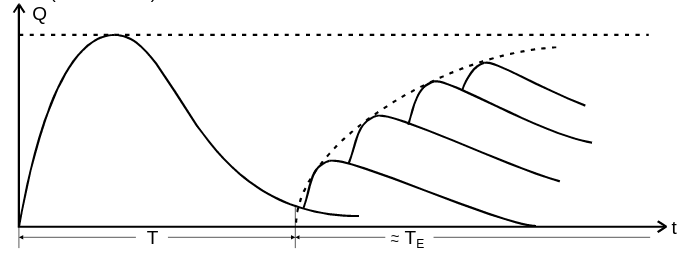
\includegraphics[width=\textwidth]{Bilder/erholzeit.png}
  \caption{Charakteristische Gestalt des Oszilloskopbild bei hohen Betriebsspannungen samt auftretender Nachentladungen. \cite{Anleitung}}
  \label{fig:nachladen}
\end{figure}

Treffen die positiven Ionen auf die Kathode, werden Elektronen aus der Metalloberfläche
losgelöst. Diese Elektronen heißen \textbf{Sekundärelektronen}. Sie durchlaufen das gesamte
Feld und haben eine genügend große Energie, um mehrere zeitlich versetzte Elektronen
zu erzeugen. Die dadurch entstehenden Impulse werden als \textbf{Nachentladungen} bezeichnet.
Diese sind unerwünscht, da sie die Registrierung eines ionisierenden Teilchens vortäuschen.
Daher wird ein Alkoholzusatz im Gas verwendet. Die positiven Ionen treffen auf die
Alkoholmoleküle und ionisieren diese aufgrund der geringeren Ionisierungsenergie von den
Alkoholmolekülen. Weiterhin gelangen die Alkoholionen zur Kathode und werden dort neutralisiert.
Allerdings werden keine Elektronen ausgelöst, sondern die Energie wird zur Anregung von
Schwingungen der Alkoholmoleküle verbraucht.
\FloatBarrier
\subsection{Charakteristik eines Zählrohres}
Die Charakteristik eines Geiger-Müller-Zählrohres ergibt sich durch Auftragen der
registrierten Teilchenzahl gegen die angelegt Spannung. Ein typischer Verlauf ist in Abbildung
\ref{fig:characteristic} dargestellt.
\begin{figure}
  \centering
  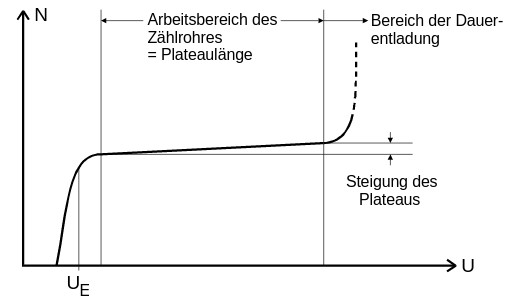
\includegraphics[width=\textwidth]{Bilder/graph_zaehlrohrcharakteristik.png}
  \caption{Charakteristischer Zusammenhang zwischen den registrierten Impulsen in Abhängigkeit zur Betriebsspannung bei konstanter Strahlungsintensität (Zählrohrcharakteristik). \cite{Anleitung}}
  \label{fig:characteristic}
\end{figure}
Der lineare Abschnitt heißt \textbf{Plateau}.
Die Länge des Plateaus ist durch den Arbeitsbereich des Geiger-Müller-Zählrohres gegeben.
Je länger das Plateau und je geringer die Steigung der Geraden ist, desto höher ist die
Qualität des Zählrohres zu bewerten.
\subsection{Bestimmung der Totzeit mit der Zwei-Quellen-Methode}
Aufgrund der Totzeit wird nicht jedes einfallende Teilchen auch registriert. Daher ist die
Zählrate der registrierten Teilchen $N_{\mathrm{r}}$ immer geringer als die Zählrate der
einfallenden
Teilchen $N_{\mathrm{w}}$. Die wahre Zählrate der einfallenden Teilchen ergibt sich zu
\begin{equation}
	N_{\mathrm{w}} = \frac{N_{\mathrm{r}}}{1-TN_{\mathrm{r}}} \, \mathrm{.}
\end{equation}
Zur Bestimmung der Totzeit $T$ wird die Zwei-Quellen-Methode verwendet.
Zuerst wird die Zählrate $N_1$ eine radioaktiven Isotops bestimmt.
Daraufhin wird ein zweites radioaktives Isotop daneben platziert und es wird die gemeinsame
Zählrate $N_{1+2}$ gemessen. Zuĺetzt wird das erste Isotop entfernt und es wird $N_2$ bestimmt.
Aufgrund der Totzeit ergibt sich die Ungleichung
\begin{equation*}
	N_{1+2} < N_1 + N_2 \, \mathrm{.}
\end{equation*}
Weiterhin lässt sich die Totzeit mit der Näherung $T^2 N_{\mathrm{i}}^2 \ll 1$ ($\mathrm{i} =
1, 2 , 1+2$) zu
%Formel die ich brauchte:
\begin{equation}
	\label{eqn:totzeit}
	T \approx \frac{N_1+N_2-N_{1+2}}{2\cdot N_1N_2}
\end{equation}
berechnen.
\subsection{Messung der pro Teilchen freigsetzten Ladungsmenge}
Ein Strommessgerät misst den mittleren Zählrohrstrom
\begin{equation}
	\bar{I} = \frac{1}{\tau} \int_0^{\tau} \frac{U(t)}{R} \symup{d}t \, \mathrm{,}
\end{equation}
wobei $\tau$ dem Messzeitintervall und $R$ dem Widerstand entspricht.
Für den Strom gilt
\begin{equation}
	\bar{I} = \frac{\Delta Q}{\Delta t} Z \, \mathrm{,}
\end{equation}
mit der in $\Delta t$ registrierten Teilchen $Z$.
Die Ladungsmenge $\Delta Q$ ist abhängig von der Spannung.
